\chapter{Understand Nodes Using Links}
\label{ch:preliminary}



In this chapter we address the first proposed research question. Namely, we use the observations in other regions and other types of data to estimate one unobserved property in focal region. We call this problem \textbf{inference problem}. At the very beginning, we give a generalized inference problem definition. Following the general definition, we look at one example of crime inference.


\section{General Problem Definition}

In this section, we give a generalized definition of the inference problem. Suppose we have a set of regions $r_1, r_2, \cdots, r_n$, and we are interested in one property $y_i$ for region $r_i$. In addition to $\vec{y}$, we also have other properties $\vec{x}_i$ observed on region $r_i$, and the set of all auxiliary properties are denoted as $X$. It is noteworthy that both $\vec{y}$ and $X$ are nodal properties. The spatial adjacency among all regions are known as $W^0$, where $W^0$ is spatial adjacency matrix. The hyperlink mobility flow is also observed as $W^k$ for type $k = \{1, 2, \cdots\}$. The entry $w_{ij}^k$ in $W^k$ refers to the quantity flow from $r_i$ to $r_j$ of type $k$.


The inference problem is that for a given region $r_t$, whose $y_t$ is unobserved, we try to use $\{y_i \} \backslash y_t$ together with $X$ and $W^k, k \in \{0, 1,2, \}$ to estimate $y_t$. Mathematically, we have
\begin{equation}
\hat{y_t} = f( \{y_i\} \backslash y_t, X, W^k),
\end{equation}
where $f$ is the estimation model of any choice.




In the next section, we will use the crime inference as  an example to show how this inference problem is solved in the literature, and how do we enhance the existing model.



\section{Crime Inference as One Example}


\begin{figure}[t]
\centering
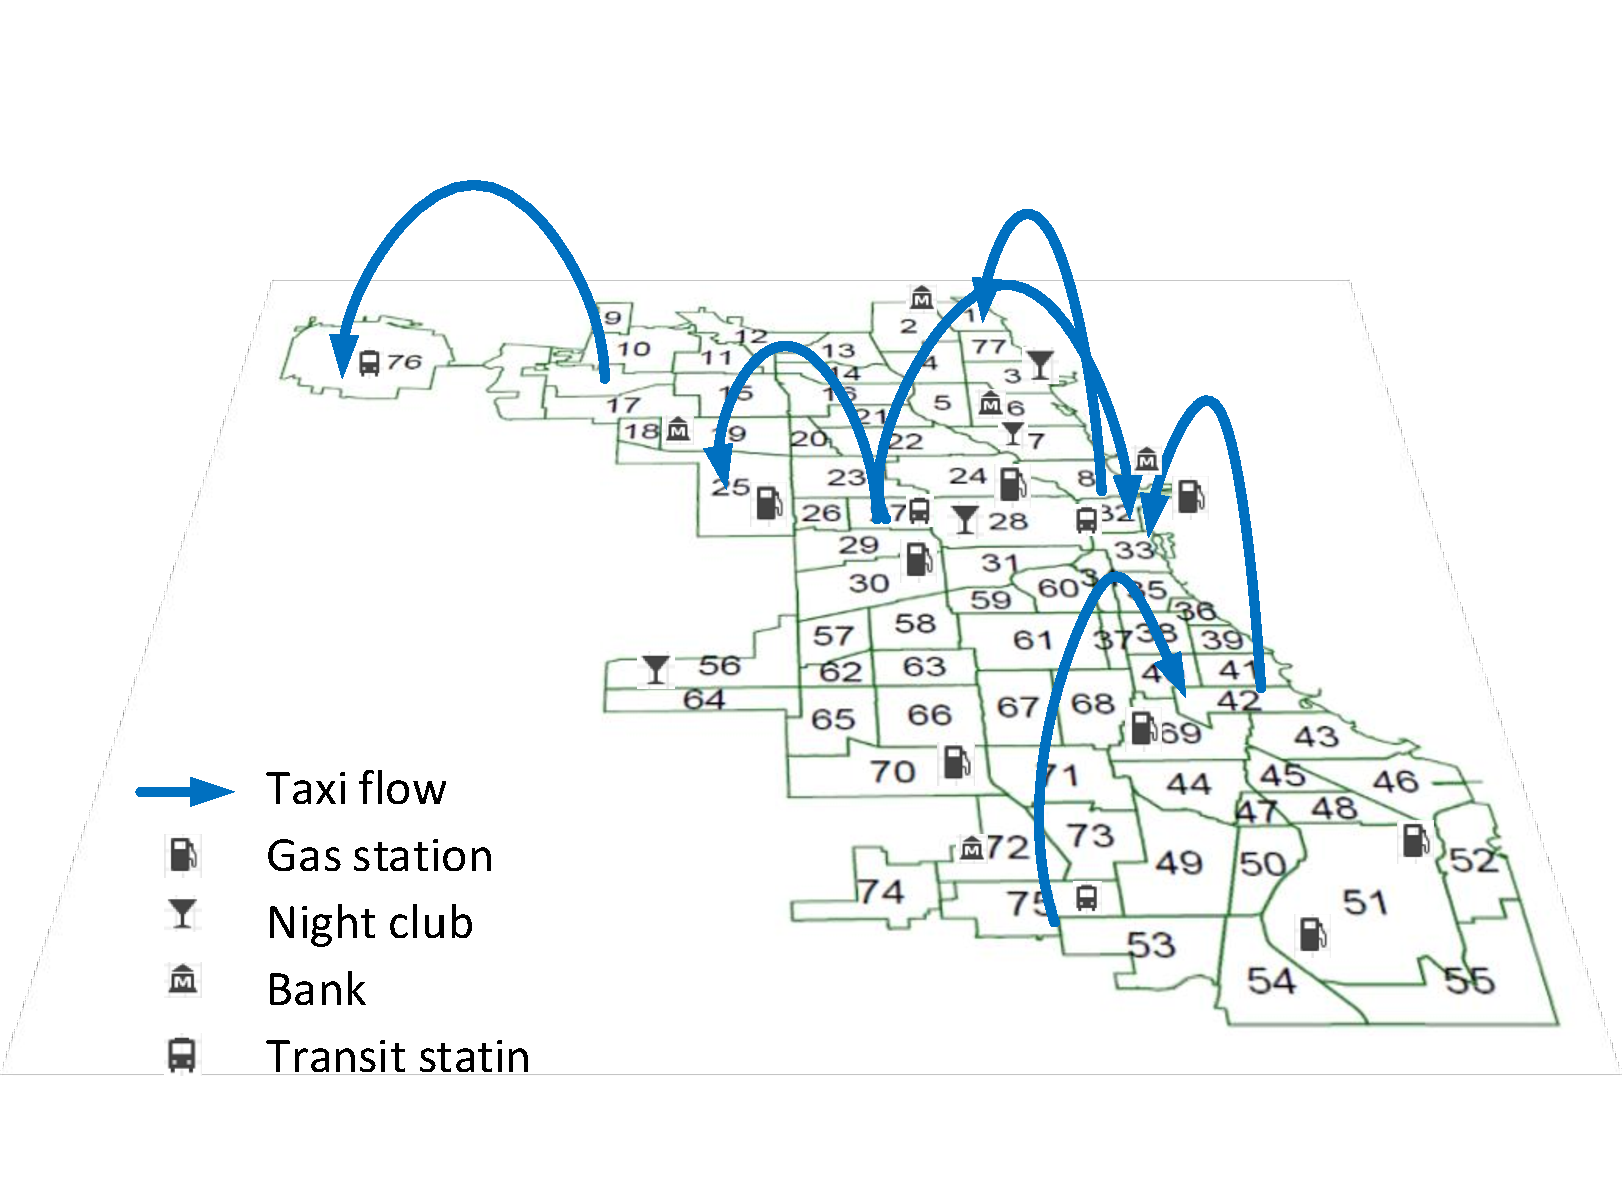
\includegraphics[width=0.8\textwidth]{fig/demo.pdf}
\caption{An illustration of various types of features we used in Chicago. The POI distribution across community areas reflects profiles of the region functionality. The taxi flow connects nonadjacent regions and act as a ``hyperlink''.}
\label{fig:demo}
\end{figure}



In Figure~\ref{fig:demo}, we show that taxi flow as a newer type of big data could provide us new insights to understand some traditional socioeconomic urban problems.  A huge amount of taxi flow data reflect how people commute in the city. In previous studies, when using geographical influence~\cite{Ans02}, people assume that a community is affected by the spatially nearby communities. However, communities are not only affected by spatially-close communities. Even if two communities are distant in geographical space, they could have a strong correlation if there are many people frequently travel between these two communities~\cite{GGM14}. We hypothesize that taxi flows may be considered as ``hyperlinks'' in the city that connect the locations and we use such data to estimate crime rates. Our experiments show very promising results --  adding taxi flow data on top of all other features can further decrease the error by 5\%.


\subsection{Related Work}


In the criminology literature researchers have studied the relationship between crime and various features. Examples are historical crime records~\cite{MSBS+12,WRWS13}, education~\cite{Ehrl75}, ethnicity~\cite{Brai89}, income level~\cite{Patt91}, unemployment~\cite{Free99}, and spatial proximity~\cite{Ans02}. 
In data mining field, newer type of data are used in the study. For example, there are works using twitter to predict crime \cite{WGB12,Gerb14}, and works using cellphone data \cite{TQC14,Bogo14} to evaluate crime and social theories at scale. 


Overall, the existing work on crime prediction can be categorized into three paradigms.



\textbf{Time-centric paradigm}. This line of work focuses on the temporal dimension of crime incidents. For example, in a study \cite{MSBS+12}, the authors propose to use a self-exciting point process to model the crime and gain insights into the temporal trends in the rate of burglary. In another study \cite{Ratc06}, the authors investigate the temporal constraints on crime, and propose an offender travel and opportunity model. This paper validates the claim that a proportion of offending is driven by the availability of opportunities presented in the offender's routine lives. 


\textbf{Place-centric paradigm}. Most existing work adopt a place-centric paradigm, where the research question is to predict the location of  crime incidents.  The predicated crime location is usually refereed by the term \emph{hotspot}, which has various geographical size.  There are plenty of works on exploration of the crime hotspots. For example, in a study \cite{TEP11} the authors  use criminal offense records to identify spatio-temporal patterns at multiple scales. They employ various quantitative tools from mathematics and physics and identify significant correlation in both space and time in the crime behavioral data.  Short \emph{et al.} \cite{SDPT+08} use a simple model to study the dynamics of crime hotspots and identify stable hotspots, where criminals are modeled as random walkers.  Bogomolov \emph{et al.} \cite{Bogo14} use human behavioral data derived from mobile network and demographic sources, together with open crime data to predict crime hotspots. They compare various classifiers and find random forest has the best prediction performance. The paper \cite{WGB12} bases on automatic semantic analysis to understand natural language Twitter posts, from which the crime incidents are reported. Some other work \cite{CTU08,ECCW05} employ the kernel density estimation (KDE) to identify and analyze crime hot spots. Those works form another form of crime prediction, which relies on the retrospective crime data to identify areas of high concentrations of crime. In  \cite{NaYa14}, the authors extend the crime cluster analysis with a temporal dimension. They employ the space-time variants of KDE to simultaneously visualize geographical extent and duration of crime clusters. 




\textbf{Population-centric paradigm}. In the last paradigm, research focuses on the criminal profiling at individual level and community level. At the individual level, \cite{WRWS13} aim to automatically  identify crimes committed by same individual from the historical crime database. The proposed system called \emph{Series Finder}, is designed to find and classify modus operandi (M.O.)  of criminals.  At the community level, Buczak \emph{et al.} \cite{BuGi10} use fuzzy association rule mining to find crime pattern. The rules they found are consistently held across all regions. The paper constructs association rules from population demographics in community.  In another paper \cite{TQC14}, the authors use computation method to validate various social theories at a large scale.  The data they used is mobile phone data in London, from which they mine the  people dynamics as features to correlate with crime.  


Our problem is different from the first two categories of work, mainly because our innovation mostly lies in using newer type of data to enhance the commonly used traditional counterpart. More specifically, we use POI to enhance the demographics information, and use taxi flow as hyper link to enhance the geographical proximity correlation. Although our problem does not consider the temporal dimension of crime in depth, it could be a promising supplement to better profile crime. Our problem dose not predict the location of any particular crime incident. Therefore the methods proposed in place-centric method are not applicable in our problem. However, the features we proposed may be incorporated in those crime prediction model. 
Our problem falls into the third paradigm,  because we are trying to profile the crime rate for Chicago community areas. In our problem, the community areas are well-defined and stable geographical regions. The newly proposed POI feature and taxi hyper link provide a unique perspective in profiling the crime rate across community areas.




\subsection{Data Description and Feature Extraction}

The crime dataset in Chicago has detailed information about the time and location (i.e., latitude and longitude) of crime and the types of crime. In our problem, when we use term crime count, we often refer to crime count in a  region (i.e., community area) in a year. The \emph{community area} is used as our geographical unit of study, since it is well-defined,  historically recognized and stable over time~\cite{wiki-ca}. In total, there are 77 community areas in Chicago.  Crime rate is the crime count normalized by the population in a region. We use vector $\vec{y} = [y_1, y_2, \ldots, y_n]$ to denote the crime rate in region $i$.


The crime data of Chicago are obtained from City of Chicago data portal~\cite{crime-data}. Chicago is the city with most complete crime data that are made public online. The crime dataset contains the incident date, location (strict name and GPS coordinates), and primary type from year 2001 to 2015. In total there are $5,856,414$ recorded crime incidents over 15 years, which is an average $390,417$ crimes incidents per year. We visualize the crime normalized by population in Figure~\ref{fig:crime-ca}, from which we can see that the downtown area has the highest crime rate.

\begin{figure}[t]
\centering
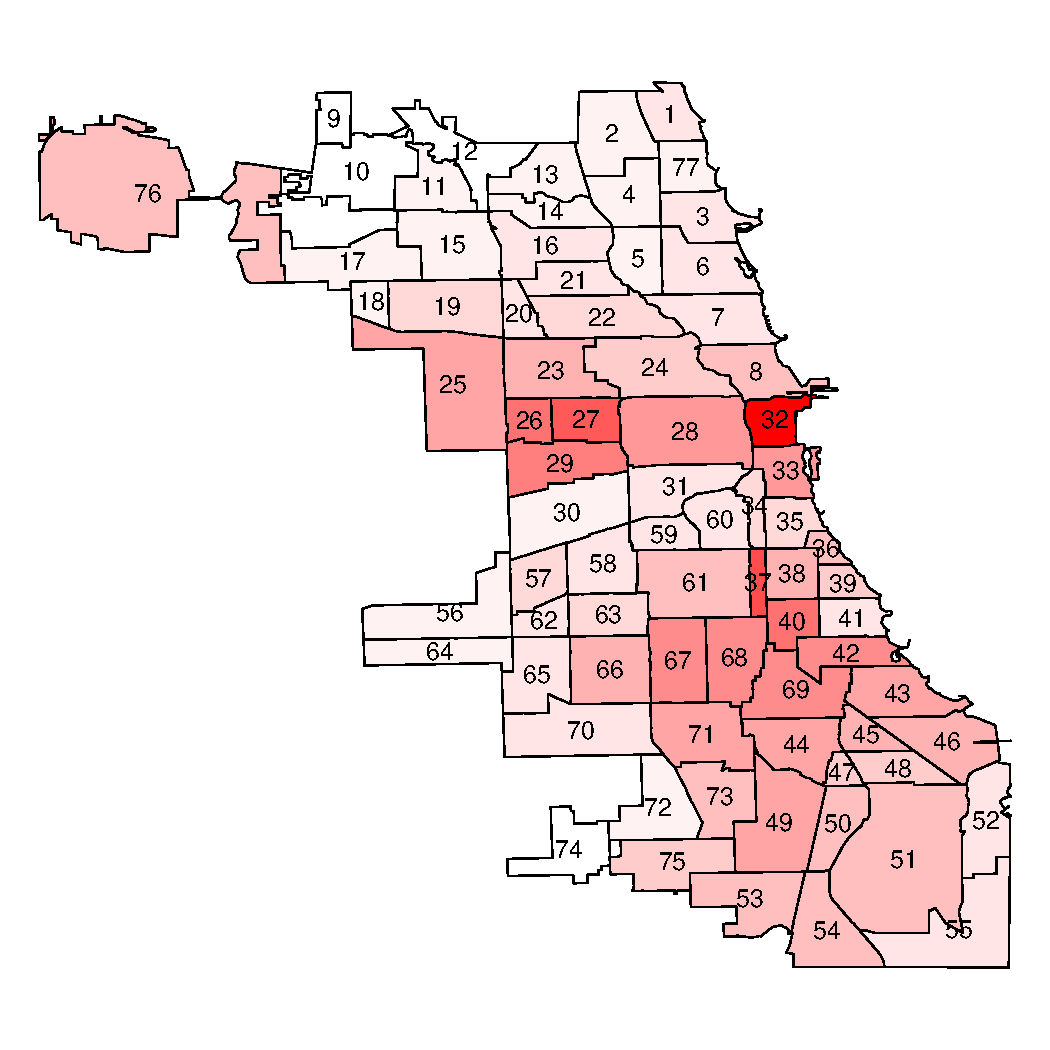
\includegraphics[width=0.7\textwidth]{fig/crime-ca.pdf}
\caption{Crime rate of Chicago by community areas. The community area \#32 is Chicago downtown, which has the highest crime rate.}
\label{fig:crime-ca}
\end{figure}


In this example we study the crime rate inference problem. More specifically, we estimate the crime rate of some regions given the information of all the other regions. Without loss of generality, we assume there is one community area $t$ with crime rate $y_t$ missing, and we use the crime rate of all the other regions $\{y_i \} \backslash y_t$ to infer this missing value. Our problem is mathematically formalized as follows
\begin{equation}
\hat{y_t} = f( \{y_i\} \backslash y_t, X),
\end{equation}
where  $X$ refers to observed extra information of  all those community areas.


\smallskip
We consider two  types of features $X$ for inference:
\begin{itemize}
\item Nodal feature. Nodal features describe the characteristics of the focal region. Such features include demographic information and Point-of-Interest (POI) distribution. Demographics are frequently used in literature, but POI is a newer type of big data, which we find significantly improve the crime inference accuracy.
\item Edge feature: (1) Geographical influence. Geographical influence considers the crime rate of the nearby locations.  This feature has been extensively used in
literature as well. To estimate the focal region, the
crime rate of nearby regions are weighted according
to spatial distances. (2) Hyperlink by taxi flow. Locations are connected through the frequent trips made by humans, which can be considered as the hyperlinks in space. This type of feature has never been studied in literature. We propose to use taxi trips to construct the social flow. Our hypothesis is that similarity in the crime rate of two regions should correlate with the social flow strength between these two regions. 
\end{itemize}



Below we will describe the datasets used to construct features and the characteristics of these features.

\begin{figure*}[t]
\centering
\subfigure[Total population]{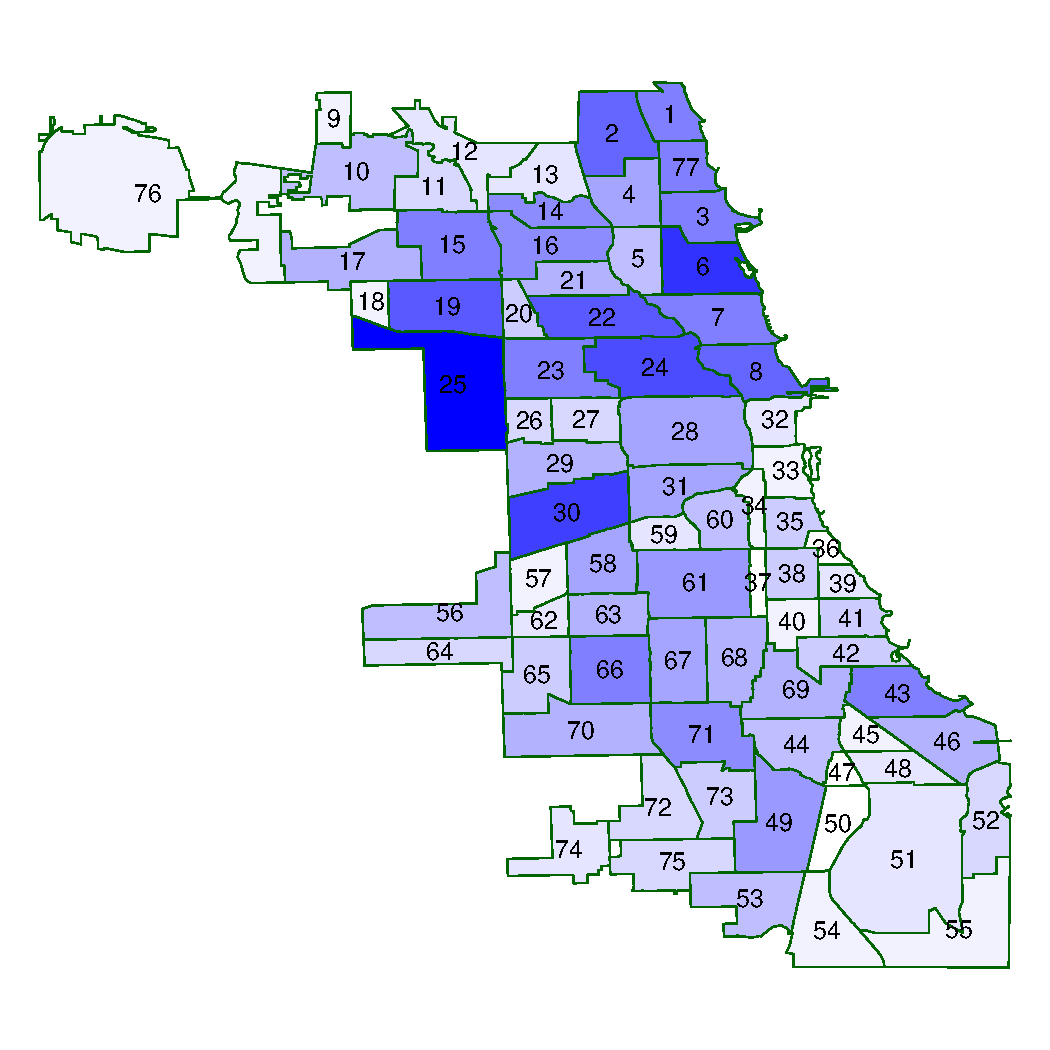
\includegraphics[width=0.45\textwidth]{fig/demo-f1.pdf}}
\subfigure[Poverty index]{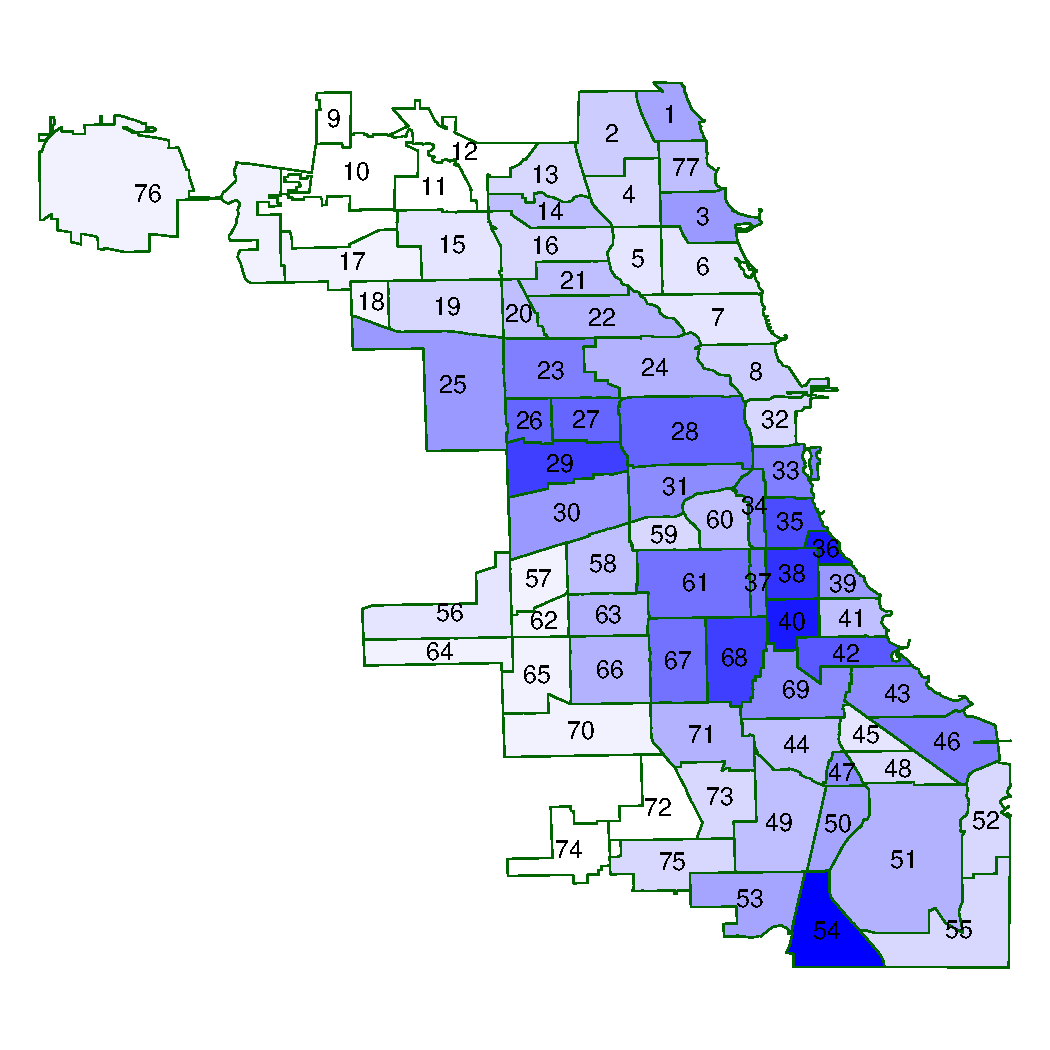
\includegraphics[width=0.45\textwidth]{fig/demo-f3.pdf}}
\subfigure[Disadvantage index]{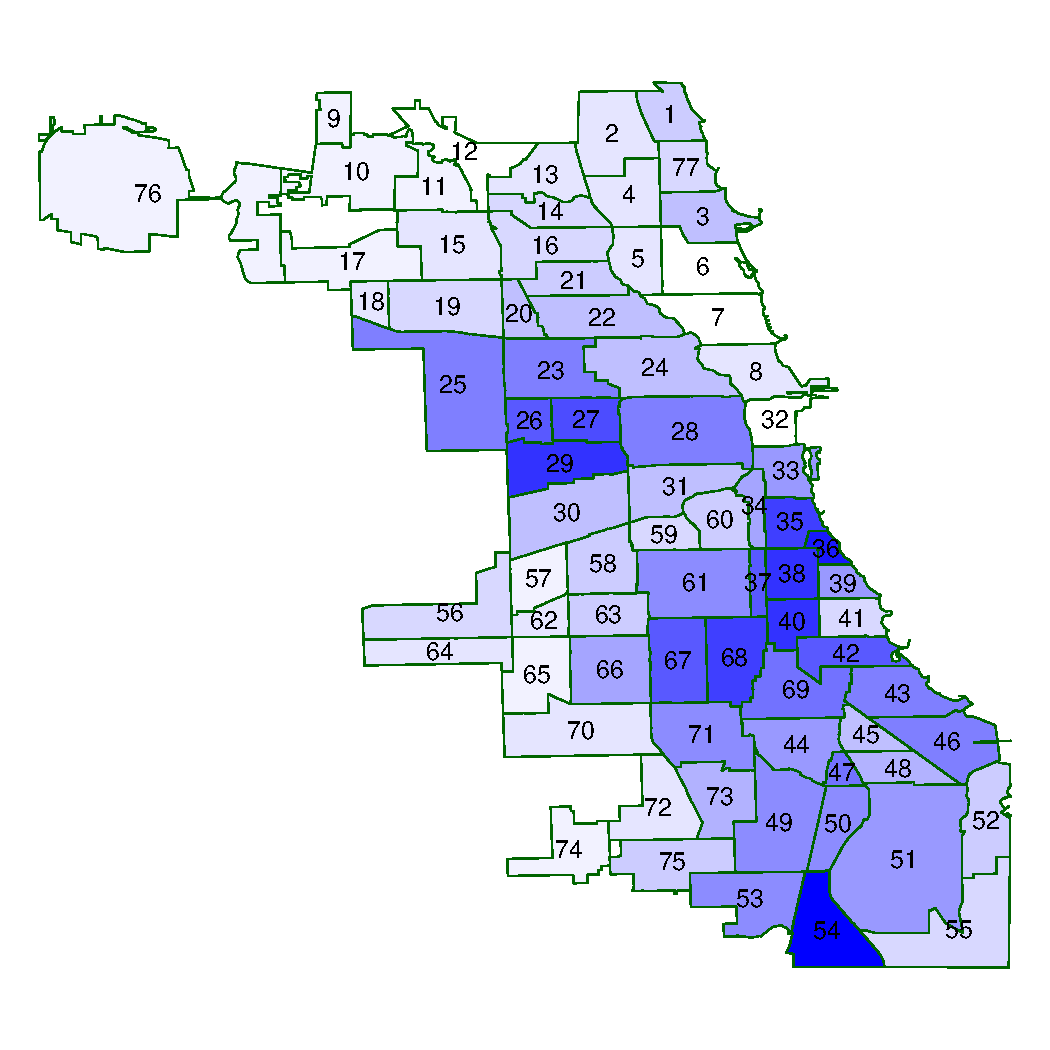
\includegraphics[width=0.45\textwidth]{fig/demo-f4.pdf}}
\subfigure[Ethnic diversity]{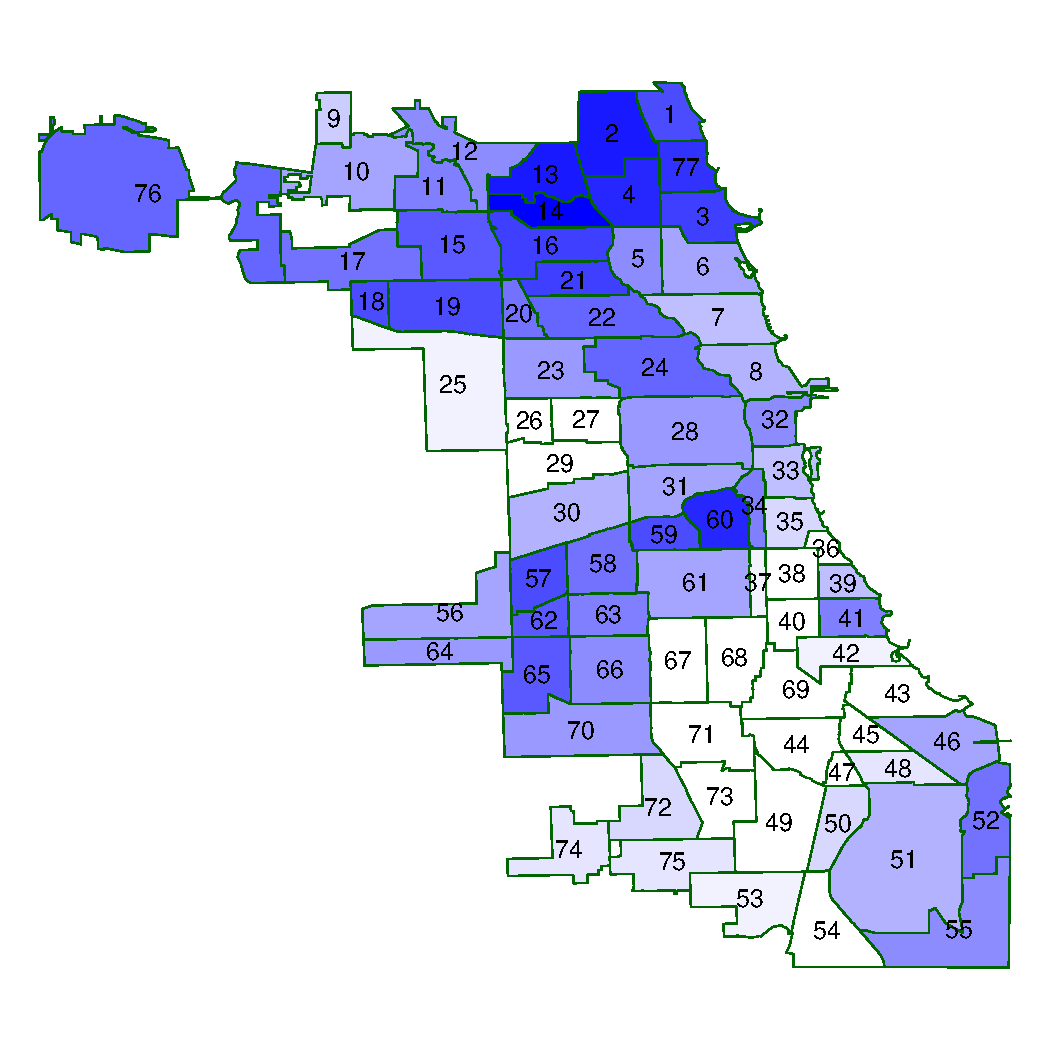
\includegraphics[width=0.45\textwidth]{fig/demo-f6.pdf}}
\caption{(a)-(d) Demographics in Chicago by community areas. Darker colors indicate higher values.}
\label{fig:demo-f}
\end{figure*}





\textbf{Nodal Feature: Demographics}

Socioeconomic and demographic features of neighborhoods have been
widely used to predict crime~\cite{Bogo14, HsPu93, WoMe12, SaHi07}. Previous studies have shown that crime rate correlates with certain demographics. For example, \cite{Jac61, GrSa09} suggests that population diversity leads to less crime in certain neighborhoods. 
In our study, we include demographic information from the US Census Bureau's Decennial Census of 2010~\cite{census-data} and American Community Survey's five-year average estimates
between 2007 and 2011. We use year 2010 data because we are evaluating crime rates in 2010-2013. The demographics include the following features:

\textsf{total population, population density, poverty, disadvantage index, residential stability, ethnic diversity, race distribution}.


The poverty index measures the proportion of community area residents
with income below the poverty level. The disadvantage index is
a composite scale based on prior work \cite{SRE97}, a function of 
poverty, unemployment rate, proportions of families with public
assistance income, and proportion of female headed households. 
 The residential stability measures home ownership and proportion of
residents who lived in the neighborhood for more than one year. Racial
and ethnic diversity is an index of heterogeneity~\cite{GrSa09} based on six
population groups, including: Hispanics, non-Hispanic Blacks, Whites,
Asians, Pacific Islanders and others.


Figure~\ref{fig:demo-f} visualizes the crime rate and demographics features in Chicago by community areas. Comparing with Figure~\ref{fig:crime-ca}, it is clear that the crime rate and poverty index and disadvantage index are consistent,  the ethnic diversity shows an inverse correlation, and the total population has little correlation with crime.



Table~\ref{tb:demo} shows the Pearson correlation coefficient between various demographics features and the crime rate at community area level. The corresponding p-value is also calculated and shown in the table to indicate the significance of the correlation coefficient.  There  are in total $77$  community areas in Chicago. Table~\ref{tb:demo} shows such correlation with several most correlated features. We can see that the poverty index and disadvantage index positively and strongly correlate with crime, while the ethnic diversity negatively correlates with crime. Other features such as total population, population density, and residential stability  have weaker correlations. One counter-intuitive observation is that the total population has a weak and negative correlation with crime. The reason is that we use crime rate in each community area, which is already normalized by the population, and therefore the total population and population density have less impact. 


\begin{table}[h]
\centering
\caption{Pearson correlation between demographic features  and crime rate (\textbf{*} indicates significant correlations with p-value less than $5\%$). }
\begin{tabular}{|c||c|c|}
\hline
Feature & Correlation & p-value \\ \hline \hline
Total Population & -0.1269 &  0.2716 \\ \hline
Population Density & -0.1972  & 0.0855 \\ \hline
Poverty Index & \textbf{0.5573*} & 1.403e-07 \\ \hline
Disadvantage Index & \textbf{0.5959*} & 1.082e-08 \\ \hline
Residential Stability  & -0.0453 &  0.6965 \\ \hline
Ethnic Diversity & \textbf{-0.5545*} &  1.678e-07 \\ \hline
Percentage of Black & \textbf{0.6696*} &  2.779e-11 \\ \hline
Percentage of Hispanic  & \textbf{-0.3820*} &  0.0006 \\ \hline
\end{tabular}
\label{tb:demo}

\end{table}







\textbf{Nodal Feature: Point-of-Interest (POI)}

While demographics are traditional census data, POI is a type of  modern data that provide fine-grained information about locations. We collect POI from FourSquare~\cite{poi-data}. POI data from FourSquare provide the venue information including venue name, category, number of check-ins, and number of unique visitors. We mainly use the major category information because categories can characterize the neighborhood functions. There are 10 major categories defined by FourSquare:

\textsf{food, residence, travel, arts \& entertainment, outdoors \& recreation, college \& education, nightlife, professional, shops, and event.}


\begin{figure}[tb]
\centering
\subfigure[Nightlife]{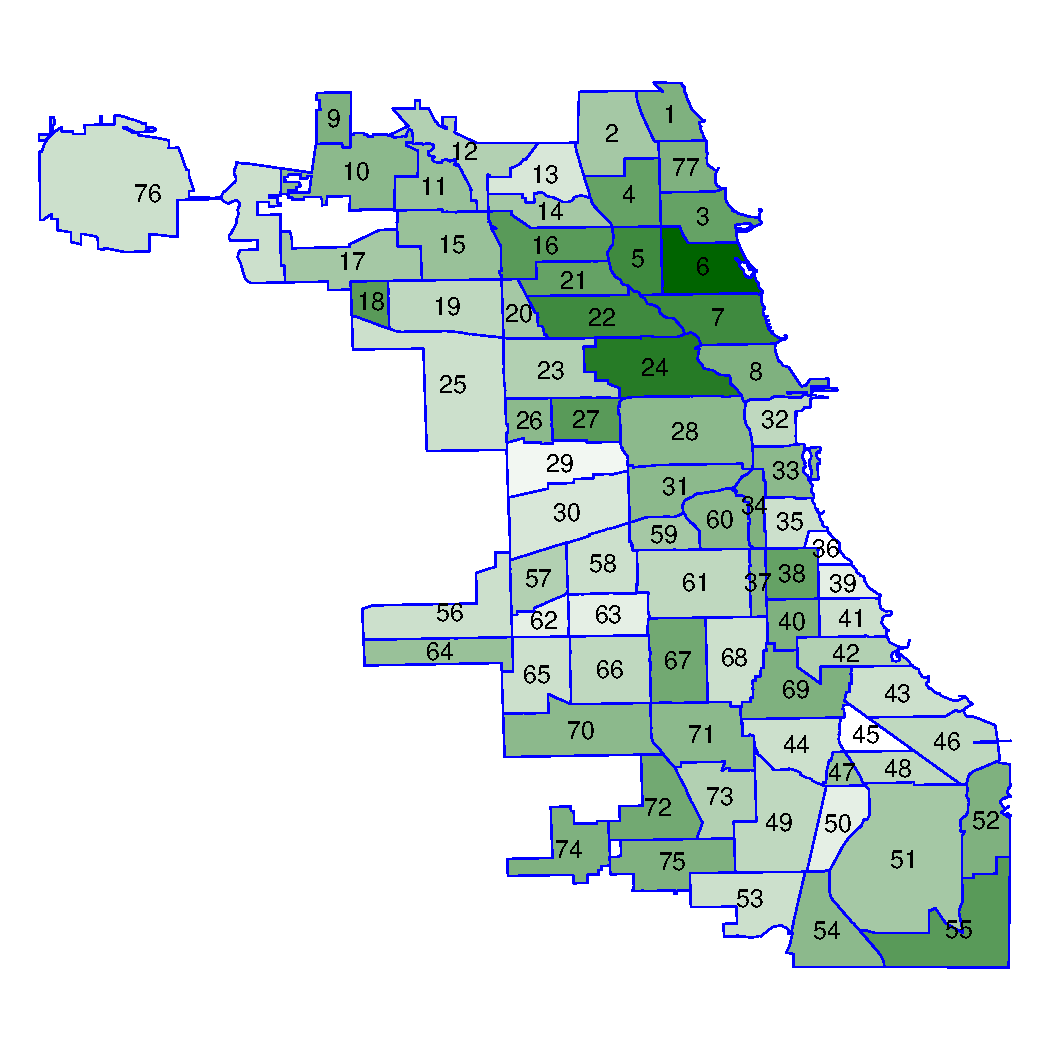
\includegraphics[width=0.45\textwidth]{fig/poi-dist7.pdf}}
\subfigure[Professional]{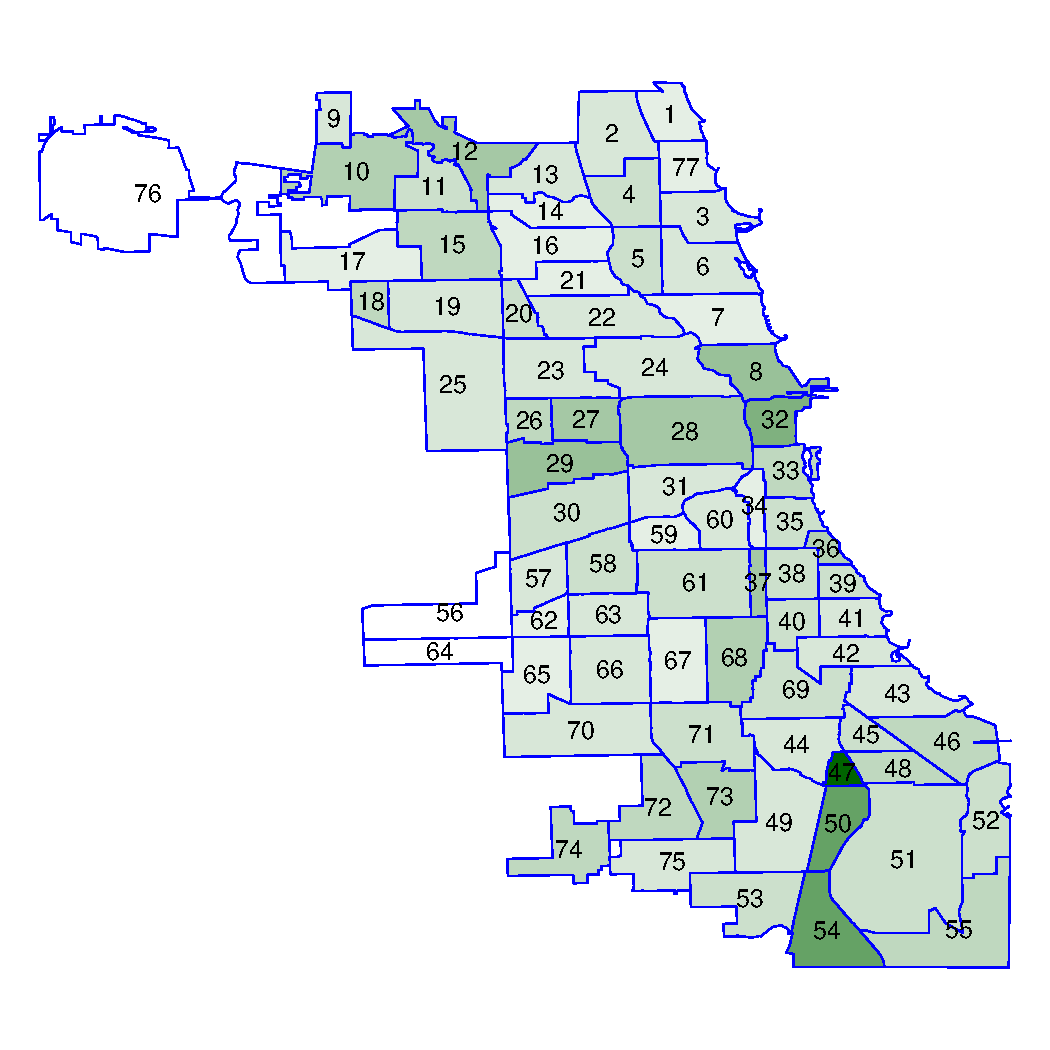
\includegraphics[width=0.45\textwidth]{fig/poi-dist8.pdf}}
\caption{Plot the  POI ratio per neighborhood. The saturation of color is proportional to the ratio value. The ``professional'' category distribution is more consistent with the crime distribution, and therefore it is the most correlated with crime. Meanwhile, the ``nightlife'' category is not positively correlated with Chicago crime.}
\label{fig:poi-coef}
\end{figure}

In total, we have crawled $112,000$  POIs from FourSquare for Chicago. Most of these POIs are in downtown area of Chicago. We normalize the POIs count per category by the total POI count in a neighborhood and plot two selected category, i.e. nightlife and professional, in Figure~\ref{fig:poi-coef}.  The darker colored neighborhoods in Figure~\ref{fig:poi-coef} are the ones with a higher portion of residence POIs.



\begin{table}[h]
\centering
\caption{Pearson correlation between POI category and crime rate (\textbf{*} indicates significant correlations with p-value less than $5\%$).}

\label{tb:poi-corr}
\begin{tabular}{|c ||c|c|}
\hline
POI category & Correlation & p-value \\ \hline \hline
Food & -0.1543 &  0.1803 \\ \hline
Residence &  -0.0610 &  0.5984 \\ \hline
Travel & -0.0017 &  0.9883 \\ \hline
Arts \& Entertainment & -0.0049 &  0.9661 \\ \hline
Outdoors \& Recreation &  0.0668 &  0.5637 \\ \hline
College \& Education & -0.0078 &  0.9473 \\ \hline
Nightlife &  -0.1553 &  0.1775 \\ \hline
Professional & \textbf{0.3221*} &  0.0043 \\ \hline
Shops & -0.1676 &  0.1450 \\ \hline
Event & 0.2196 &  0.0549  \\ \hline
\end{tabular}
\end{table}



In Table~\ref{tb:poi-corr} we show the Pearson correlation between POI category and crime rate. The category ``professional''  is most significantly correlated with the crime rate. Under the professional POI category, there are some venues with a large population concentration, such as transportation center, convention center, community center, and co-working space. In those venues, the  population volume is high and residential stability is low, therefore the professional POI counts positively correlates with crime rate.  One counter-intuitive observation is that ``nightlife'' category is not positively correlated with crime ($-0.1553$). This can be explained through Figure~\ref{fig:poi-coef}(a). The majority of nightlife venues in Chicago locate in northern area, while most crime incidents occur in downtown area.








\textbf{Edge: Geographical Influence}

Together with the US census demographics data, we also collected the boundary shape files of Chicago, which are used to calculate the geographical influence feature.

Previous studies have also shown that the crime rate at one location is highly correlated with nearby locations~\cite{GSGL01, Bur88}. Such geographical influence is also frequently used in the literature~\cite{ACC00, MoSa97}, which is calculated as:
\begin{equation}
\vec{F^g} = W^g \cdot \vec{Y},
\label{eq:spatial}
\end{equation}
where $W^g$ is the spatial weight matrix. If region $i$ and $j$ are not geospatially adjacent, $w_{ij}^g = 0$; otherwise, $w_{ij}^g \propto distance(i,j)^{-1}$.

\begin{figure}[t]
\centering
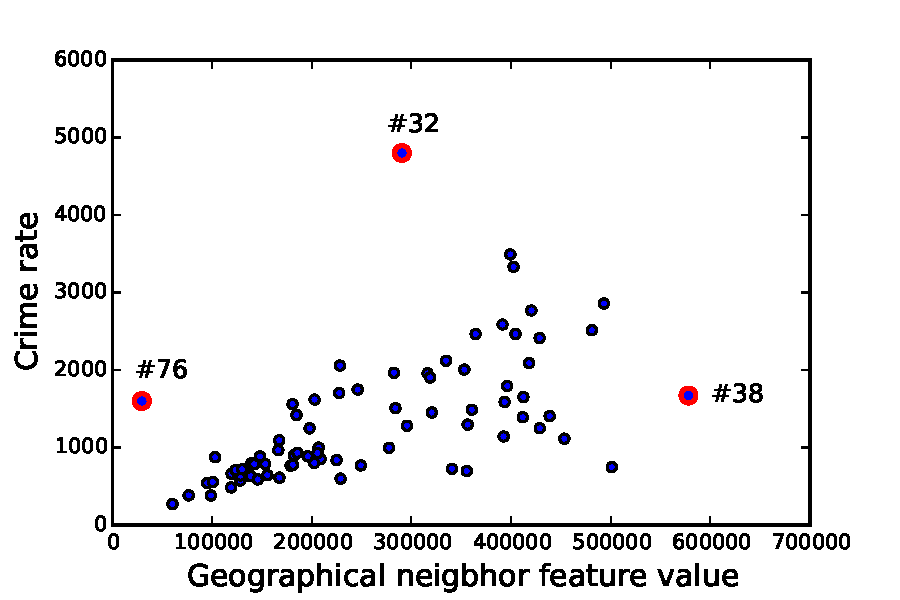
\includegraphics[width=0.8\textwidth]{fig/spatial-crime-rate.pdf}
\caption{The geographical influence feature correlation with crime. In the plot we marked out three outliers and their corresponding community area ID.}
\label{fig:spatial}
\end{figure}

In Figure~\ref{fig:spatial},  we plot crime rate with respect to geographical influence calculated in Eq.~\ref{eq:spatial}. We observe an obvious positive correlation, which means if nearby neighborhoods have a high crime rate, the focal neighborhood is more likely to have a high crime rate. We also do observe a few outliers in Figure~\ref{fig:spatial}. These neighborhoods show different crime rate in their nearby neighborhoods compared to their own. For example, as we can also see in Figure~\ref{fig:crime-ca}, community area \#38 locates in an area where the the neighbors have high crime rates but its crime rate is relatively low; in contrast, neighborhood \#32 has a high crime rate even though its neighbors have relatively low crime. The community area \#76 home of the O'Hare International Airport is far from most of other community areas, however its own crime rate is relative high.





\textbf{Edge: Hyperlinks by Taxi Flow}

In our Chicago taxi dataset, there are $1,048,576$ taxi trips in total during the October to December in 2013. For each trip the following information are available: pickup/dropoff time, pickup/dropoff location, operation time, and total amount paid. We requested the taxi trip records from Chicago taxi commission pursuant of the Freedom of Information Law.  Figure~\ref{fig:taxi-flow} shows a visualization of the major flows at community level.

\begin{figure}[htb]
\centering
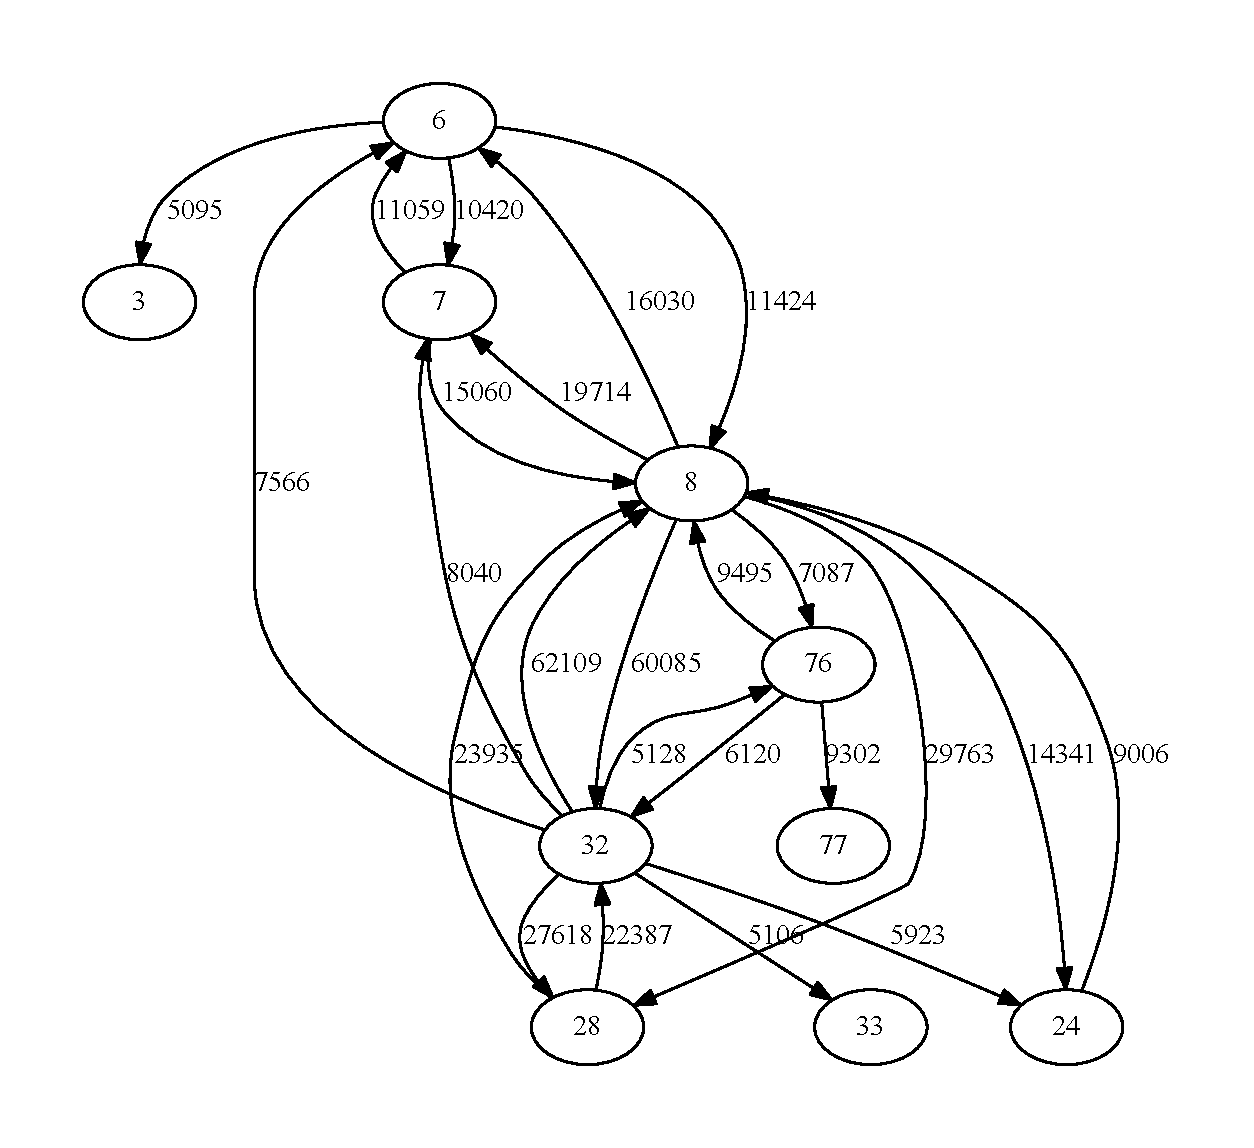
\includegraphics[width=0.8\textwidth]{fig/taxiflow.pdf}
\caption{Major taxi flows between neighborhoods. We set a threshold ($> 5,000$) on the flow and only plot the high volume flow. The label on the node is the ID of the corresponding community areas. We can see that there are several hub community areas, such as \#6, \#8, \#32, which are all in the downtown areas. The label on the edge shows how many taxi trips are commuting through the two community areas for three months in 2013.}
\label{fig:taxi-flow}
\end{figure}


One of our hypothesis is that the social interaction among two community areas propagates crime from one region to another.
The Chicago taxi data captures the social interactions among various community areas. To calculate this first, we first map all taxi trips to community areas to get the taxi flow $w_{ij}\ \forall i,j \in \{1, 2, \cdots n\}$. Then the taxi flow lag is constructed by the product of social flow and the crime rate of neighboring regions as follows
\begin{equation}
\vec{F^t} = W^t \cdot \vec{Y}.
\label{eq:taxi}
\end{equation}
The taxi flow $W^t$ is a matrix with entry $w_{ij}$ denoting the taxi flow from $i$ to $j$. Note that $\forall i$, $w^s_{ii} = 0$ in matrix $W^t$, because we have to exclude the crime in focal area from its own predictor. The semantic of this taxi flow feature is how many crime in the focal area is contributed by its neighboring areas through social interaction.

The correlation between taxi flow and crime rate is shown in Figure~\ref{fig:taxi-corr}. From the scatter plot, we can see that overall the crime rate is positively correlate with the taxi flow. There are two  outliers clearly shown in Figure~\ref{fig:taxi-corr}. The community area \#32 is the downtown Loop, which has the highest crime rate and is hard to predict by taxi flow. Another anomalous community area \#47 has relatively low crime rate by itself. However, this area has a lot of in flows from high-crime communities. 




\begin{figure}[ht]
\centering
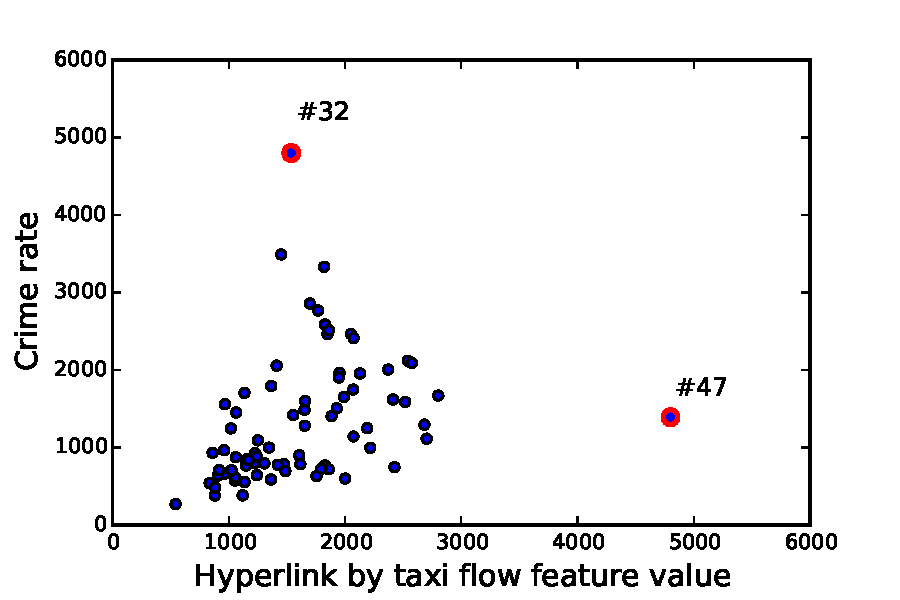
\includegraphics[width=0.8\textwidth]{fig/taxi-flow-percent.pdf}
\caption{Correlation between taxi flow and crime rate. In the plot, we marked out three outliers and their corresponding community area ID.}
\label{fig:taxi-corr}
\end{figure}






\subsection{Spatial Autoregressive Inference Model}



\textbf{Linear Regression}

The most straightforward prediction is linear regression model. This model assumes the error terms follow a Gaussian distribution $\epsilon \sim \mathcal{N}(0, \sigma^2)$. As a result the parameter distribution also follows a Gaussian distribution. This assumption makes the model less generative, since in real applications, there is no way to ensure the dependent variable has a Gaussian error term. 


Equation~\ref{eq:lrm} gives the linear regression formulation of our problem.
\begin{equation}
\label{eq:lrm}
\vec{y} = \vec{\alpha}^T \vec{x} + \beta^f W^f \vec{y} + \beta^g W^g \vec{y} + \vec{\epsilon},
\end{equation}
where $\vec{x}$ represents the nodal features including demographics and POI distribution, $W^f$ is the flow matrix of taxi flow, and $W^g$ is the spatial matrix representing the geographical adjacency. On the right-hand side, $\epsilon$ is the only stochastic variables, and all other terms are fixed observation values. Therefore, we incorporate all the fixed observations into one term $X$, and we get the standard regression problem
\[
E(y) = X w + \epsilon.
\]


In order to learn the regression parameter $w$, we can use a maximum likelihood estimator. Since $\epsilon = y - Xw$, the joint probability of error term is
\begin{equation}
P(\epsilon | w) = \frac{1}{\sqrt{2\pi \sigma^2}} e^{-\frac{(y - Xw)^2}{2 \sigma^2}}.
\end{equation}
Maximizing the joint probability gives us the optimal solution.



\textbf{Linear regression gives negative prediction}

One obvious drawback is that the linear regression is not a count prediction model, since it will give negative number as prediction. For example, we find the suspicious community \#32 case. Refer to Figure~\ref{fig:crime-ca}, we know this community is the downtown. The crime count for community \#32 is $7,709$ in 2010. However, the linear regression base model gives $-1,448$ as prediction. This result is not acceptable in a count prediction model. We further look into the features of community \#32 to figure out why it has negative crime count estimation. It turns out that community \#32 has $12,175$ venues in total, which is 10 times more than the average of other communities ($1,011$). In our learned model, the venue count feature has a negative coefficients, which indicates that popular places tend to have less crime incidents. The big difference in the venue count feature lead to a negative prediction for community \# 32.




\textbf{Poisson regression as a count prediction model}

To address this issue, a count prediction model is a natural selection. The \emph{Poisson regression} is another form of regression, more appropriate for count data than linear regression \cite{GMS95}\cite{Lamb92}. With shortened notation $X$, Poisson regression model has the exponential function as link function
\begin{equation}
\label{eq:prm}
E(y) = e^{X w}.
\end{equation}
This comes from the assumption that $y$ follows Poisson distribution with mean $\lambda $. Additionally, the mean $lambda$ is determined by observed independent variables $X$, with the link function $\lambda = e^{Xw}$. Adding all together, the joint probability of $y$ is 
\begin{equation}
P(y|w) = \frac{e^{-e^{Xw}}(e^{Xw})^y}{y!}.
\end{equation}


Compared with the linear regression, the negative log-likelihood function of Poisson regression is derived from the dependent variable itself, unlike linear regression, which is derived from the joint distribution of error term. 


However, Poisson regression enforces the mean and variance of dependent variable $y$ to be equal. This restriction leads to the ``over-dispersion'' issue for some real problems, that is the presence of larger variability in data set than the statistical model expected. In our crime dataset, the mean of crime count for all communities is $4,787$, while the variance is $1.6 \times 10^7$. The variance is almost the square of the mean, which significantly violate the Poisson distribution assumption. Therefore, we should look for other count prediction model.




\textbf{Negative binomial regression addresses over-dispersion}

To allow larger variance in the predicted value,  we introduce the Poisson-Gamma mixture model, which is also known as \emph{negative binomial regression}.  The negative binomial regression has been used in similar work~\cite{Osg00}.




Given that the crime rate $y$ follows Poisson distribution with mean $\lambda$.  In order to allow for larger variance, now the $\lambda$ itself is a random variable, distributed as a Gamma distribution with shape $k=r$ and scale $\theta = \frac{1-p}{p}$.  The probability function of $y$ becomes
\begin{align}
P(y| r, p) & = \int_0^{\infty} P_{Poisson}(y|\lambda) \cdot P_{Gamma}(\lambda|r, p) d \lambda \nonumber \\ 
		& = \int_0^{\infty} \frac{\lambda^y}{y!} e^{-\lambda} \cdot \lambda^{r-1} \frac{e^{-\lambda(1-p)/p}}{(\frac{p}{1-p})^y \Gamma(r)} d\lambda  \nonumber \\
		& = \frac{\Gamma(r+y)}{y! \Gamma(r)} p^k (1-p)^y
\end{align}
This is exactly the probability density function of negative binomial distribution.


In negative binomial regression, the link function is
\begin{equation}
E(y) = e^{X w + \epsilon}.
\end{equation}
The error term $e^\epsilon$ is the mixture prior, and we assume it follows Gamma distribution with shape parameter $k=\frac{1}{\theta}$, so that it has mean $E(e^\epsilon) = k\theta = 1$ and variance $Var(e^\epsilon) = k\theta^2 = \theta$. This setting ensures the $E(y) = e^{Xw} \cdot e^\epsilon = e^{Xw}$.





\subsection{Evaluation of negative binomial regression model}



\textbf{Evaluation Settings}

We adopt the leave-one-out evaluation to estimate the crime rate of one geographic region given all the information of all the other regions. When we construct the spatial/social lag variable for the training data, the effect of testing region is completely removed. For example, if region $y_t$ is the testing region, the remaining $\{y_i\} \backslash y_t$ become the training set. For any $y_j$ in the training set, its geographical influence feature and taxi flow feature are constructed from $\{y_i\} \backslash \{y_t, y_j\}$.


In the evaluation, we estimate the crime rate for testing community area. The accuracy of estimation is evaluated by mean absolute error (MAE) and mean relative error (MRE).

\begin{align}
MAE & = \frac{\sum_i^n |y_i - \hat{y_i}| }{n} \\
MRE & = \frac{\sum_i^n |y_i - \hat{y_i}|} {\sum_i^n y_i }
\end{align}


\textbf{Performance Study: Negative Binomial Regression vs. Linear Regression}


We evaluate the estimation accuracy under various feature combinations. The leave-one-out evaluation results are shown in Table~\ref{tb:perf}.  We run both linear regression model and negative binomial model on five consecutive years, 2010 -- 2014. Both MAE and MRE are shown in the table. We have four types of features, demographics, POI, geographical influence and taxi flow. We test the various settings of feature combinations.





\begin{table}[htb]
\centering
\caption{Performance evaluation. Various feature combinations are shown in each column. The linear regression model and negative binomial results are compared by year group. }

\label{tb:perf}
\begin{tabular}{|c|c|c|c|c|c|c|c|c|c|c|}
\hline
\multicolumn{3}{|c|}{} & \multicolumn{8}{|c|}{Settings} \\ \hline
\multicolumn{3}{|c|}{Column ID} & 1 & 2 & 3 & 4 & 5 & 6 & 7 & 8 \\ \hline
\multicolumn{2}{|c|}{\multirow{4}{*}{Features$^1$}}	& D & \checkmark & \checkmark&\checkmark & \checkmark & \checkmark& \checkmark& \checkmark& \checkmark \\ \cline{3-11}
\multicolumn{2}{|c|}{}	& G & & & & & \checkmark & \checkmark& \checkmark& \checkmark \\ \cline{3-11}
\multicolumn{2}{|c|}{}	& P & & \checkmark & & \checkmark & &\checkmark & & \checkmark \\ \cline{3-11}
\multicolumn{2}{|c|}{}	& T & & & \checkmark& \checkmark & & & \checkmark& \checkmark \\ \hline
Year & Model$^2$ & Error & \multicolumn{8}{|c|}{} \\ \hline
	\cellcolor{white}&  \cellcolor{white} & MAE & 394.41 & 416.98 & 408.09 &  406.93  &394.78 &432.45 & 402.25& 416.41\\ \cline{3-11}
	&	\multirow{-2}{*}{LR}& MRE & 0.294& 0.311 & 0.304 & 0.304 & 0.295 &0.323 & 0.300& 0.310\\ \cline{2-11}
	\rowcolor{Gray}
	\cellcolor{white}	& \cellcolor{white} & MAE & 391.53&   333.14 & 395.64 & 323.47 & 389.55&350.06 & 387.43& \textbf{320.75}\\ \cline{3-11}
	\rowcolor{Gray}
	\cellcolor{white}\multirow{-4}{*}{2010}	&\cellcolor{white}\multirow{-2}{*}{NB}	& MRE & 0.292& 0.249 & 0.295 & 0.241 & 0.290& 0.261& 0.289& \textbf{0.239} \\ \hline
	


	\cellcolor{white}	& \cellcolor{white} & MAE & 380.22&   409.30 & 396.97 &  401.11 & 379.61& 422.94&389.39 & 408.91\\ \cline{3-11}
	&	\multirow{-2}{*}{LR}& MRE &0.295  &  0.318  &  0.309 &  0.312 & 0.295 &0.328 & 0.302 & 0.320   \\ \cline{2-11}
	\rowcolor{Gray}
	\cellcolor{white}& \cellcolor{white} & MAE &381.11 & 332.62 & 388.81  & 328.94 & 378.84& 345.24& 381.33& \textbf{335.97} \\ \cline{3-11}
	\rowcolor{Gray}
	\cellcolor{white}\multirow{-4}{*}{2011}	&	\cellcolor{white}\multirow{-2}{*}{NB}& MRE&0.296 & 0.259 & 0.302  & 0.256 & 0.294 & 0.268  & 0.296  & \textbf{0.253}  \\ \hline
	


	\cellcolor{white}& \cellcolor{white} & MAE &378.91 & 412.95 & 401.54  & 412.20& 376.53 & 423.88 & 399.25 & 419.93\\ \cline{3-11}
	&	\multirow{-2}{*}{LR}& MRE& 0.306 & 0.334 & 0.325 & 0.333&  0.304 & 0.343 & 0.322 & 0.339 \\ \cline{2-11}
	\rowcolor{Gray}
	\cellcolor{white}& \cellcolor{white} & MAE & 386.31 & 337.24 & 389.58  & 331.41 & 384.23 & 352.22 & 381.67 & \textbf{345.49} \\ \cline{3-11}
	\rowcolor{Gray}
	\cellcolor{white}\multirow{-4}{*}{2012}&\cellcolor{white}\multirow{-2}{*}{NB}	& MRE& 0.312 & 0.273 & 0.315  & 0.268 & 0.310 & 0.284 & 0.308 & \textbf{0.279} \\ \hline
	

	\cellcolor{white}& \cellcolor{white} & MAE & 367.89 & 420.81 & 390.75  & 402.75 & 369.24 & 433.48 &388.92 & 412.31\\ \cline{3-11}
	&	\multirow{-2}{*}{LR}& MRE& 0.324 &  0.370 & 0.344  & 0.354  & 0.325 & 0.381 & 0.342& 0.362\\ \cline{2-11}
	\rowcolor{Gray}
	\cellcolor{white}& \cellcolor{white}& MAE & 376.08&  333.92 & 373.08 & 312.63 & 377.57 & 350.33 & 368.49 & \textbf{319.86}\\ \cline{3-11}
	\rowcolor{Gray}
	\cellcolor{white}\multirow{-4}{*}{2013}	&	\cellcolor{white}\multirow{-2}{*}{NB} & MRE& 0.331 &   0.294 & 0.328  & 0.275 & 0.332 & 0.308 & 0.324& \textbf{0.281}\\ \hline

	\cellcolor{white}& \cellcolor{white} & MAE & 331.28 & 375.53 & 349.00  & 350.31 & 329.93& 386.90& 345.79& 361.28\\ \cline{3-11}
	&	\multirow{-2}{*}{LR} & MRE& 0.326 & 0.369 & 0.343  & 0.345 & 0.324& 0.380& 0.340& 0.355\\ \cline{2-11}
	\rowcolor{Gray}
	\cellcolor{white}&\cellcolor{white}  & MAE & 340.73 & 293.52  & 339.17  & 274.45 & 336.09& 308.18& 326.07& \textbf{273.27}\\ \cline{3-11}
	\rowcolor{Gray}
	\cellcolor{white}\multirow{-4}{*}{2014}	&	\cellcolor{white}\multirow{-2}{*}{NB}& MRE& 0.335&  0.289 & 0.334 & 0.270 &  0.331 & 0.303& 0.321 & \textbf{0.269}\\ \hline
\end{tabular}

\footnotesize{$^1$ D -- demographic features, G -- geographical influence, P -- POI features, T -- taxi flow feature.\\}
\footnotesize{$^2$ LR -- Linear Regression, NB -- Negative Binomial Regression.}
\end{table}




We compare the estimation error of negative binomial model with the linear regression base model. We use a incremental settings, where new features are added on top of previous one. The results are shown in Figure~\ref{fig:lrvsnb}.


\begin{figure}[h]
\centering
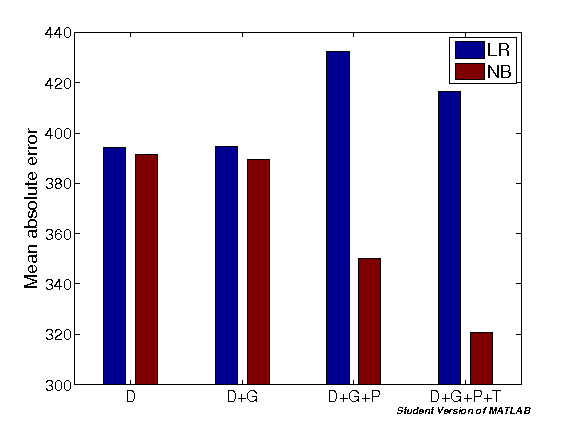
\includegraphics[width=0.8\textwidth]{fig/lrvsnb.png}
\caption{The inference error for linear regression base model. $^*$D -- demographic features, G -- geographical influence, P -- POI features, T -- taxi flow feature}
\label{fig:lrvsnb}
\end{figure}



It is clear that the negative binomial model significantly outperform the linear regression model. Meanwhile, the negative binomial model captures our intuition well. Namely, adding new features will effectively improve the estimation accuracy.


In Table~\ref{tb:perf},  we can see that in different years and under most settings, the negative binomial regression significantly outperforms the linear regression (with only a few exceptions when using only demographic feature). When using all the features, NB is significantly better than LR with at least $6\%$ improvement in relative error.
One reason is that the negative binomial is a count prediction model, which assumes some distribution for the predicted variable and guarantee its positivity. Another reason is that it is difficult to get very precise estimation of crime rate, and  negative binomial model allows a large variance in the estimated crime rate. Therefore negative binomial is more appropriate for crime rate estimation than linear regression.





\section{Conclusion}


In this chapter, we discuss the a general inference problem that using information on the links to understand the nodes.


We extend the spatial autoregressive model in the literature by adding new types of flow into the model.  We call this model flow augumented spatial autoregressive model. This modification makes it impossible to use standard T-test to get the significance of the model coefficients. Therefore, we use the Monte-Carlo tests, where a repeated leave-one-out schemes is designed.


The flow augumented spatial autoregressive model has its own weakness, which will be discussed in next chapter. In the next chapter, we presents the unified graphical model to model the interactions.
